\documentclass{article}

\usepackage{amsmath}
\usepackage{amssymb}
\usepackage{amsthm}
\usepackage[margin = 2.54cm]{geometry}
\usepackage{tikz}

\newtheorem{lemma}{Lemma}
\newtheorem{definition}[lemma]{Definition}
\newtheorem{prop}[lemma]{Proposition}

\begin{document}
We start with a lemma.
\begin{lemma}[Exchanging the order of integration]\label{lemma:1}
  If $f(x)$ is smooth enough, we have
  \begin{equation}
    \int_0^a \!\!\! \int_0^x
    f(x, y) \, \mathrm{d} y \, \mathrm{d} x =
    \int_0^a \!\!\! \int_{y}^a
    f(x, y) \, \mathrm{d} x \, \mathrm{d} y,
  \end{equation}
  where $a \ge 0$.
\end{lemma}
The `proof' can be shown in Figure~\ref{fig:lemma-1}.
\begin{figure}[htbp]
  \centering
  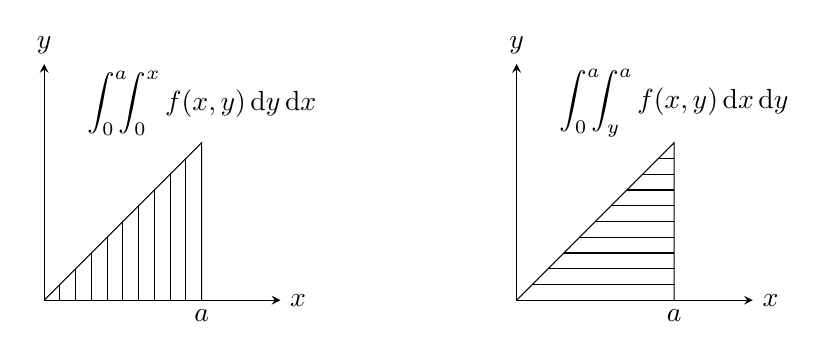
\begin{tikzpicture}[>=stealth, scale=2]
    \newcommand\kX{1}
    \newcommand\kN{10}
    \begin{scope}[shift={({-1.5 * \kX}, 0)}]
      \draw[<->]
        (0, {1.5 * \kX}) node[above]{$y$} --
        (0, 0) --
        ({1.5 * \kX}, 0) node[right]{$x$};
      \draw
        (0, 0) --
        (\kX, \kX) --
        (\kX, 0);
      \draw (\kX, 0) node[below]{$a$};
      \foreach \x in {1,...,\kN} {
        \draw
          ({\kX / \kN * \x}, {\kX / \kN * \x}) --
          ({\kX / \kN * \x}, 0);
      }
      \draw ({1.0 * \kX}, {1.25 * \kX}) node
        {$\displaystyle
        \int_0^a \!\!\! \int_0^x
        f(x, y) \, \mathrm{d} y \, \mathrm{d} x$};
    \end{scope}
    \begin{scope}[shift={({1.5 * \kX}, 0)}]
      \draw[<->]
        (0, {1.5 * \kX}) node[above]{$y$} --
        (0, 0) --
        ({1.5 * \kX}, 0) node[right]{$x$};
      \draw
        (0, 0) --
        (\kX, \kX) --
        (\kX, 0);
      \draw (\kX, 0) node[below]{$a$};
      \foreach \x in {1,...,\kN} {
        \draw
          ({\kX / \kN * \x}, {\kX / \kN * \x}) --
          (\kX, {\kX / \kN * \x});
      }
      \draw ({1.0 * \kX}, {1.25 * \kX}) node
        {$\displaystyle
        \int_0^a \!\!\! \int_{y}^a
        f(x, y) \, \mathrm{d} x \, \mathrm{d} y$};
    \end{scope}
  \end{tikzpicture}
  \caption{`Proof' of Lemma~\ref{lemma:1}.}
  \label{fig:lemma-1}
\end{figure}

And a definition.
\begin{definition}[The integrator $I$]
  $I_a^b f(x)$ is defined as
  \begin{equation}
    I_a^b f(x) \mathrel{:=} \int_a^b f(x) \, \mathrm{d} x.
  \end{equation}
\end{definition}

Then comes the proposition.
\begin{prop}[Multiple integration]
  If $f(x)$ is smooth enough, we have
  \begin{equation}
    I_n f(x) \mathrel{:=}
    I_0^{x_0} \prod_{i = 1}^n (I_0^x) f(x) =
    \int_0^{x_0} \frac{(x_0 - x)^n}{n!} f(x) \, \mathrm{d} x,
  \end{equation}
  where $n \in \mathbb{N}$.
\end{prop}
\begin{proof}
  First, the proposition holds for $n = 0$.
  Then we assume it holds for $n = k$,
  and we have
  \[\begin{aligned}
    I_{k + 1} f(x) =
    I_k \bigl( I_0^x f(x) \bigr) &=
    \int_0^{x_0} \frac{(x_0 - x)^k}{k!}
    \biggl( \int_0^x f(t) \, \mathrm{d} t \biggr)
    \, \mathrm{d} x \\
    &= \int_0^{x_0} \!\!\! \int_0^x
    \frac{(x_0 - x)^k}{k!} f(t)
    \, \mathrm{d} t \, \mathrm{d} x \\
    &= \int_0^{x_0} \!\!\! \int_t^{x_0}
    \frac{(x_0 - x)^k}{k!} f(t)
    \, \mathrm{d} x \, \mathrm{d} t \\
    &= \int_0^{x_0}
    \frac{(x_0 - t)^{k + 1}}{(k + 1)!} f(t)
    \, \mathrm{d} t \\
    &= \int_0^{x_0}
    \frac{(x_0 - x)^{k + 1}}{(k + 1)!} f(x)
    \, \mathrm{d} x. \qedhere
  \end{aligned}\]
\end{proof}
\end{document}